\section{Introduction}

Model predictive control (MPC) has received an explosion of interest in recent decades \cite{Mayne2014}, and in particular the use of \emph{nonlinear} prediction models presents significant and unique challenges \cite{Grune2011}. While the use of linearized plant models in model predictive control can lead to poor performance or instability if nonlinear dynamics are strong enough, we must also avoid the construction of complex nonlinear models whose associated optimization problems are highly non-convex or computationally unfeasible~\cite{Mayne1996}.

In this chapter, the application of MPC to nonlinear Volterra series models will be considered. The system prediction models are assumed to be in the form of Laguerre basis function expansions, for which the standard time domain Volterra series is a special case. Robust identification of Volterra-Laguerre models was discussed in Chapter \ref{chap:5} of this thesis, where the proposed method could, in theory, estimate the series up to an arbitrarily large nonlinear order. However, the use of such models in model-based control is problematic, since there are no existing results on the use of high order Volterra-Laguerre models for this purpose. There has been some work published on feedback control and MPC using the time domain series \cite{Doyle2002}, but with no formal controller derivations for Volterra series order higher than three. The use of basis function expanded models has been similarly limited to the second order case \cite{Parker1998}, \cite{Parker2002}.  

The contributions of this chapter are as follows. Firstly, a summary of previous achievements in Volterra series model-based control is provided. A flexible nonlinear state space representation is proposed for the arbitrary order Volterra-Laguerre model structure, using Kronecker algebra to define the nonlinear output mapping. A Volterra-Laguerre MPC algorithm is then developed using a typical quadratic objective function. When the move horizon is limited to 1 (i.e. constant over the prediction horizon), the MPC optimization is shown to be reduced to a problem of finding and evaluating polynomial roots, regardless of the model's series order. Extensions to the algorithm are also developed which can handle input constraints and remove steady-state tracking errors. The stability properties of the algorithm are explored, and the relationship between the input penalty term and control stability is discussed in detail.

\section{History of Volterra series model-based control}

In the 1990s, results began to appear in the control theory literature which used Volterra series models and their variants for control design. Some of the first methods to be developed for Volterra series model-based control were proposed in \cite{Maner1994} and \cite{Doyle1995}, with a more complete discussion later included in \cite{Doyle2002}. The methods rely on a decomposition of the Volterra series into its linear and nonlinear components, such that the input/output relationship can be expressed as
\begin{equation}
y = (\mathbf{L}+\mathbf{N}) [u]
\label{eqn:LinNonlinOperator}
\end{equation}
where $\mathbf{L}$ is the linear operator corresponding to first order Volterra kernel $h_1$, and $\mathbf{N}$ is the nonlinear operator built from constant, $h_0$, and higher order kernels, $h_2$, $h_3$, etc. Model-based control typically utilizes an approximate inverse of the plant to decide the control action, and a rearrangement of the operator in (\ref{eqn:LinNonlinOperator}) will produce the inverse expression:
\begin{equation}
(\mathbf{L}+\mathbf{N})^{-1} = (\mathbf{I} + \mathbf{L}^{-1}\mathbf{N})^{-1} \mathbf{L}^{-1}.
\label{eqn:LinNonlinInverse}
\end{equation}
The expression on the right hand side of (\ref{eqn:LinNonlinInverse}) is easily shown to be realized by the feedback structure in Figure \ref{fig:LinNonlinInvRealization}. Thus, only the linear kernel is required to be (approximately) inverted, which was already a standard task in linear model-based control at the time of development. Combining this model inverse with the typical filters required for realizability and robustness, an effective controller could be designed. 

\begin{figure}[h]
\centering
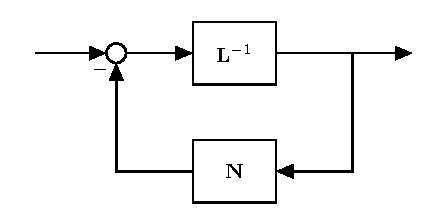
\includegraphics[scale = 1]{Chapter10_NMPC/VolterraIMC.pdf}
\caption{Negative feedback structure which can be used to realize the inverse of a plant with linear and nonlinear components}
\label{fig:LinNonlinInvRealization}
\end{figure}

The model-based control results in \cite{Doyle1995} have been applied to a number of practical control problems, including glucose levels in a simulated diabetic patient \cite{Rubb2004}, polymerization processes \cite{Maner1996}, \cite{Li2005}, the temperature of a greenhouse \cite{Gruber2011} and airflow in a fuel cell \cite{Gruber2012}. In each of these problems, the Volterra series model was limited to the second order or a simplified third order structure, as these are the only orders at which analytic results are available for the control design, and no regularized methods existed for robust identification of more complex higher order models. 

The use of Laguerre expansions has also been discussed in the literature for Volterra series model-based control. Indeed, Volterra-Laguerre models were applied in adaptive control as early as 1993, in \cite{Dumont1993}. The basis function approach is attractive for the same reasons which were highlighted for identification in Chapter \ref{chap:5}, namely that an appropriate choice of the basis functions can result in a dramatic reduction in the number of parameters required to describe the system. A model-based predictive controller for second order Volterra-Laguerre models was described in \cite{Dumont1994}, and extended in \cite{Parker1998}, where it was applied to a bioreactor process. The method relies on a simplified state space model for the second order series, which neglects the constant kernel $h_0$, and restricts all kernels to the same Laguerre basis for expansion. Further extensions to the control design were provided in \cite{Parker2002}, to accommodate larger move horizons, and in \cite{Antoine2006}, for two-input/two-output systems. None of these methods are able to be extended to models with a higher series order. 

\section{A flexible state space representation}

In this section, a nonlinear state space model will be developed for the Volterra series expanded by Laguerre basis functions. The model should be flexible enough to consider a separate basis at each nonlinear order of the series, and the constant kernel contribution should be included. The standard formulation for such a model (\ref{OBFvolterra}), is repeated in (\ref{OBFvolterra_Chap10}) for convenience,
\begin{equation}
\begin{split}
\label{OBFvolterra_Chap10}
y^0(t) &= \alpha_0 + \sum_{m=1}^{M} y_m(t), \\
y_m(t) &= \sum_{i_1=1}^{\mathcal{B}_m} \hdots \sum_{i_m=1}^{\mathcal{B}_m} \alpha_m(i_1,\hdots,i_m) \prod_{j=1}^{m} u^f_{m,i_j}(t).
\end{split}
\end{equation}
Recall that $u^f_{m,l}(t)$ refers to a filtered version of the input, $u(t)$, where the filter is the $l$\textsuperscript{th} basis function of the $m$\textsuperscript{th} order basis. Laguerre basis functions are used in this chapter, where the filters are given in the $z$-domain by
\begin{equation}
\label{LBFdef_Chap10}
F_{m,l}(z) = \frac{\sqrt{1-|a_m|^2}}{z-a_m} \bigg( \frac{1-a_m z}{z-a_m} \bigg) ^{l-1}, \; \; \; a_m \in (-1,1).
\end{equation}

To express the arbitrary order Laguerre-expanded model (\ref{OBFvolterra_Chap10}) in a state space framework, it will be necessary to define the Kronecker product and its associated exponent.

\begin{defn}[Kronecker product]
The Kronecker product of two matrices, $X \in \mathbb{F}^{s \times t}$ and $Y \in \mathbb{F}^{u \times v}$, is defined as 
\begin{equation}
X \otimes Y = \begin{bmatrix} X(1,1) \cdot Y & \hdots & X(1,t) \cdot Y \\ \vdots & \ddots &\vdots \\ X(s,1) \cdot Y & \hdots & X(s,t) \cdot Y \end{bmatrix} \in \mathbb{F}^{su \times tv},
\end{equation}
where $X(i,j)$ denotes the $i,j$\textsuperscript{th} element of matrix $X$, and $\mathbb{F}$ is an arbitrary field.
\end{defn}

\begin{defn}[Kronecker exponent]
The Kronecker exponent of a matrix $X$ is denoted by $[X]^{\otimes m}, \; m \in \mathbb{N}$, and defined as $m-1$ repeated Kronecker products of $X$ with itself, i.e. 
\begin{equation}
[X]^{\otimes m} = X \underbrace{\otimes X \otimes \hdots \otimes X}_{m-1 \text{ products}}
\end{equation}
Special cases are defined analogously to the scalar exponent: $[X]^{\otimes 1} = X$ and $[X]^{\otimes 0} = 1$.
\end{defn}

Another function involving the Kronecker product will also be defined for use in the MPC derivation.

\begin{defn}[Kronecker permutation-sum function]
For arbitrary matrices $X_1,X_2,\hdots,X_m$, the function $\mathcal{K}_m(X_1,X_2,\hdots,X_m)$ is defined as the sum, over all unique orderings of the matrix arguments, of the total Kronecker product of all arguments. For example, $$\mathcal{K}_3(X,Y,Y) = X \otimes Y \otimes Y + Y \otimes X \otimes Y + Y \otimes Y \otimes X.$$
\label{def:Kronpermsum}
\end{defn}

\begin{rem}
It is useful to note that $\mathcal{K}_m(X,X,\hdots,X) = [X]^{\otimes m}$.
\end{rem}

Additionally, a vectorization operator is defined, that will be applied to the basis function kernels, $\alpha_m(i_1,\hdots,i_m)$, in the state space model.

\begin{notation}[$\vect(\cdot)$ operator]
For any $m$-dimensional tensor, $X(i_1,\hdots,i_m) \in \mathbb{R}^{N \times \hdots \times N}$, the operator $\vect(X)$ is defined as the standard vectorization operator. A row vector output convention will be used for $\vect(\cdot)$ in this chapter.
\end{notation}

Now a state space model can be constructed to capture the expressions (\ref{OBFvolterra_Chap10}) and (\ref{LBFdef_Chap10}). Rather than using a single state vector, individual state vectors will be defined for each nonlinear order, $m$. The state vector, $x_m(t)$, at a given order contains appropriate Laguerre filtered inputs at sample $t$, i.e.
\begin{equation}
x_m(t) = \begin{bmatrix} u^f_{m,1}(t) & u^f_{m,2}(t) & \hdots & u^f_{m,\mathcal{B}_m}(t) \end{bmatrix}^T.
\end{equation} 

The full state space model can now be expressed as follows,
\begin{align}
x_m(t+1) &= A_m x_m(t) + B_m u(t), \; \; m = 1,2,\hdots,M, \label{eqn:SS_dynamic_VL}\\
y^0(t) &= \alpha_0 + \sum_{m=1}^M \vect(\alpha_m) \cdot \big[ x_m(t) \big]^{\otimes m}. \label{eqn:SS_output_VL}
\end{align} 
The state equation (\ref{eqn:SS_dynamic_VL}) is seen to be split into independent linear equations for each state vector. The matrices $A_m$ and $B_m$ at each order should be constructed so as to carry out the Laguerre filtering operation at that order, i.e.
\begin{align}
A_m &= \begin{bmatrix} a_m & 0 &0 & \hdots &0 \\ r_m &a_m & 0 & \hdots &0 \\ -a_m r_m &r_m &a_m & \hdots &0 \\ \vdots & \vdots & \vdots & \ddots & \vdots \\ (-a_m)^{q_m-2}r_m & (-a_m)^{q_m-3}r_m & \hdots & r_m & a_m\end{bmatrix}, \\
B_m &= \sqrt{r_m} \cdot \big[1 \; \; -a_m \; \; a_m^2 \; \; \hdots \; \; (-a_m)^{\mathcal{B}_m-1} \big]^T,
\end{align}
with $r_m = 1-a_m^2$. 

In the output equation, (\ref{eqn:SS_output_VL}), there is a static nonlinear map from the state vectors to the model output, $y^0$. For each nonlinear order, $m$, multiplication of the vectorized basis function kernel with a Kronecker exponent of the state vector allows every $m$\textsuperscript{th} order state product to be matched with its corresponding expansion coefficient.

\begin{rem}
The model developed here in (\ref{eqn:SS_dynamic_VL}) and (\ref{eqn:SS_output_VL}) is a more flexible representation than the Volterra-Laguerre state space structure used in \cite{Parker1998} and \cite{Parker2002}. Firstly, here the maximum nonlinear order is not limited to $M=2$, and can be made arbitrarily large using the Kronecker algebra framework. Furthermore, a separate basis can be used for each nonlinear order, since expanding all Volterra kernels with the same Laguerre basis is almost always suboptimal from an accuracy standpoint \cite{Campello2004}. Finally, the constant kernel contribution, $\alpha_0$, is explicitly considered here.
\end{rem}

\section{Model predictive control design}

A model predictive controller will be designed in this section using the proposed state space Volterra-Laguerre model. The prediction horizon, $p$, for the scheme is left arbitrary here, however the move horizon is fixed at $\mu = 1$, i.e. the input is assumed constant within the prediction window during each objective optimization. This is not without precedent, as similar restrictions were imposed in \cite{Parker1998} and \cite{Antoine2006}. The move horizon is restricted such that the MPC optimization problem is able to be solved in a computationally efficient manner, as will become clear in the sequel. We consider a typical quadratic objective function, which for $\mu =1$ can be written as,
\begin{align}
\label{eqn:MPC_ObjFn_Chap10}
&\min_{u(t)} \Bigg\{ \sum_{j=1}^{p} [y^0(t+j|t) - r(t)]^2  + \Gamma_u \big[ u(t) - u(t-1) \big]^2 \Bigg\} \\
&\textrm{subject to } u(t+j) = u(t) \; \; \forall j \in 1,2,\hdots,p. \nonumber
\end{align}
The objective contains two penalty terms. The first term penalizes the difference between the output and desired reference $r(t)$ over the prediction horizon. The second term penalizes large input changes, and the relative dominance of this term can be scaled using the design parameter $\Gamma_u$. The input penalty term is typically included for reasons of robustness.

\subsection{State space prediction model}

Given the $\mu = 1$ move horizon restriction adopted in the objective function, the state space model in (\ref{eqn:SS_dynamic_VL}) and (\ref{eqn:SS_output_VL}) can be easily modified to allow prediction of the output at any future sample time within the prediction window. The prediction model for this case can be expressed as,
\begin{align}
x_m(t+j) &= A_m^j x_m(t) + \bar{A}_m^{(j)} B_m u(t) \; \; \; m = 1,2,\hdots,M, \label{eqn:SS_dynamicpredict_VL}\\
y^0(t+j) &= \alpha_0 + \sum_{m=1}^M \vect(\alpha_m) \cdot \big[ x_m(t+j) \big]^{\otimes m}  \label{eqn:SS_outputpredict_VL},
\end{align}
where $j>0$ is the number of samples forward in the prediction from the current sample, $t$, and $\bar{A}_m^{(j)} = (A_m^{j-1} + A_m^{j-2} + \hdots + I)$.

\subsection{Minimizing the objective function}

In order to choose the control input at any given sample, $t$, the objective function (\ref{eqn:MPC_ObjFn_Chap10}) should be minimized. Denoting this optimal input by $u^*(t)$, we have that
\begin{align}
\label{eqn:MPC_ObjFn2_Chap10}
u^*(t) = &\text{arg } \min_{u(t)} \Bigg\{ \sum_{j=1}^{p} [y^0(t+j|t) - r(t)]^2  + \Gamma_u \big[ u(t) - u(t-1) \big]^2 \Bigg\} \; \; \forall t.
\end{align}

Now, noting that the minimizer $u^*(t)$ will correspond to a stationary point of the objective function in (\ref{eqn:MPC_ObjFn2_Chap10}), and introducing the shorthand notation,
\begin{equation}
X_j = y^0(t+j|t) - r(t),
\label{eqn:Xj_shorthand}
\end{equation}
we have that
\begin{align}
&u^*(t) \in   \Bigg\{ u(t): \frac{\partial}{\partial u(t)} \Bigg( \sum_{j=1}^{p} \big[ X_j \big] ^2  + \Gamma_u \big[ u(t) - u(t-1) \big]^2 \Bigg) = 0 \Bigg\}\\
\implies &u^*(t) \in \Bigg\{ u(t): \sum_{j=1}^{p} X_j \cdot \frac{\partial}{\partial u(t)} X_j  + \Gamma_u \big[ u(t) - u(t-1) \big] = 0 \Bigg\}. \label{eqn:MPC_ObjFn3_Chap10}
\end{align}

Examining first the term $X_j = y^0(t+j|t) - r(t)$, and substituting the prediction equations (\ref{eqn:SS_dynamicpredict_VL}) and (\ref{eqn:SS_outputpredict_VL}) into (\ref{eqn:Xj_shorthand}), it can be seen that $X_j$ is a polynomial in $u(t)$ of order $M$,
\begin{equation}
X_j = \gamma_{M,j} \big[ u(t) \big]^M + \hdots + \gamma_{2,j} \big[ u(t) \big]^2 + \gamma_{1,j} u(t) + \gamma_{0,j}
\end{equation}
where the polynomial coefficients are given by,
\begin{equation}
\begin{split}
\gamma_{0,j} &= \alpha_0 + \sum_{m=1}^M \vect(\alpha_m) \cdot \big[ A_m^j x_m(t) \big]^{\otimes m} - r(t)\\
\gamma_{1,j} &= \sum_{m=1}^M \vect(\alpha_m) \cdot \mathcal{K}_m (\bar{A}_m^{(j)}B_m,\underbrace{A_m^j x_m(t),\hdots,A_m^j x_m(t)}_{m-1 \text{ times}}) \\
\gamma_{2,j} &= \sum_{m=2}^M \vect(\alpha_m) \cdot \mathcal{K}_m (\bar{A}_m^{(j)}B_m, \bar{A}_m^{(j)}B_m, \underbrace{A_m^j x_m(t),\hdots,A_m^j x_m(t)}_{m-2 \text{ times}}) \\
& \; \; \vdots \\
\gamma_{M,j} &= \vect(\alpha_m) \cdot \big[ \bar{A}_M^{(j)}B_M \big]^{\otimes M},
\label{eqn:MPC_gammacoeffs}
\end{split}
\end{equation}
and where $\mathcal{K}_m(\cdot)$ is the function introduced in Definition \ref{def:Kronpermsum}. Thus, the term $X_j \cdot \frac{\partial}{\partial u(t)} X_j$ will also be polynomial,
\begin{equation}
X_j \cdot \frac{\partial}{\partial u(t)} X_j = \beta_{2M-1,j} \big[ u(t) \big]^{2M-1} + \hdots + \beta_{2,j} \big[ u(t) \big]^2 + \beta_{1,j} u(t) + \beta_{0,j},
\label{eqn:XjdXj_poly}
\end{equation}
where the $\beta_{i,j}$ coefficients can be obtained from a convolution of the $X_j$ coefficient vector with its vector of derivatives, i.e.
\begin{equation}
\begin{split}
[\beta_{2M-1,j} , &\beta_{2M-2,j} , \hdots ,\beta_{1,j} ,\beta_{0,j}] \\
&= [\gamma_{M,j} , \gamma_{M-1,j} , \hdots , \gamma_{0,j}] * [M \gamma_{M,j} , (M-1) \gamma_{M-1,j} , \hdots , \gamma_{1,j}].
\label{eqn:MPC_betacoeffs}
\end{split}
\end{equation} 
Now substituting (\ref{eqn:XjdXj_poly}) into (\ref{eqn:MPC_ObjFn3_Chap10}), we obtain a final result for the objective function minimizer,
\begin{equation}
\begin{split}
u^*(t) \in   \Bigg\{ u(t): \Big\{ &\sum_{j=1}^{p} \beta_{2M-1,j} \Big\} \big[ u(t) \big]^{2M-1} + \hdots + \Big\{ \sum_{j=1}^{p} \beta_{2,j} \Big\} \big[ u(t) \big]^2 \\
&+ \Big\{ \sum_{j=1}^{p} \beta_{1,j} + \Gamma_u \Big\} u(t) + \Big\{ \sum_{j=1}^{p} \beta_{0,j} - \Gamma_u u(t-1) \Big\} = 0 \Bigg\}
\label{eqn:MPC_finalminimizer}
\end{split}
\end{equation}

We can see from (\ref{eqn:MPC_finalminimizer}) that for a move horizon $\mu=1$, the MPC optimization problem reduces to finding the roots of a scalar polynomial, and then evaluating each root in the objective function (\ref{eqn:MPC_ObjFn_Chap10}) to identify the global minimizer $u^*(t)$. The function evaluations are computationally trivial, and the root-finding task can also be performed in a computationally efficient manner. One common approach to root-finding is to replace the polynomial by its corresponding companion matrix, and compute the eigenvalues of the matrix using established methods such as power iteration or the QR algorithm~\cite{Francis1961}, \cite{Kublanovskaya1962}.
\begin{rem}
In practice, the controller input is a strictly real quantity, hence only the strictly real roots from the set in (\ref{eqn:MPC_finalminimizer}) need to be considered. Furthermore, since the polynomial order ($2M-1$) is guaranteed to be odd, there exists at least one strictly real root.
\end{rem}

Having derived a solution methodology for the Volterra-Laguerre MPC objective function, the proposed control scheme is summarized in Algorithm \ref{alg:BasicVL-MPC}.

\begin{algorithm}[h]
\begin{algorithmic}[1]
\Require $\Gamma_u$, $p$, $r(t)$, initial condition $u(-1)$, state space model parameters $A_m, B_m, \alpha_m$ %for $m = 1,2,\hdots,M$
\State $t \gets 0$
\While{Control is running} 
\ForAll{$j \in 1,2,\hdots,p$}
\State Compute the $X_j$ polynomial coefficients using (\ref{eqn:MPC_gammacoeffs}) 
\State Compute the $X_j \cdot \frac{\partial}{\partial u(t)} X_j$ coefficients using (\ref{eqn:MPC_betacoeffs}) 
\EndFor
\State Compute the coefficients of the minimizer polynomial in (\ref{eqn:MPC_finalminimizer})
\State Find all roots of the minimizer polynomial in (\ref{eqn:MPC_finalminimizer})
\State Evaluate the objective function (\ref{eqn:MPC_ObjFn_Chap10}) for all strictly real roots
\State Choose $u^*(t)$ as the root which produced the lowest objective function value
\State Apply $u^*(t)$ to the physical system
\State $t \gets t+1$
\EndWhile
\end{algorithmic}
\caption{MPC scheme for Volterra-Laguerre models }
\label{alg:BasicVL-MPC}
\end{algorithm}

\subsection{Handling input constraints}

Thus far, we have neglected the existence of input constraints in the formulation of our MPC objective function, while actuator limitations always exist in practice. In order to prevent the MPC scheme from selecting input values which violate such practical limits, modifications to the algorithm are necessary. Here we will consider the case in which the input is constrained to a particular closed region of the total scalar space, such that the constrained MPC objective function is
\begin{align}
\label{eqn:MPC_ConstrainedObjFn_Chap10}
&\min_{u(t)} \Bigg\{ \sum_{j=1}^{p} [y^0(t+j|t) - r(t)]^2  + \Gamma_u \big[ u(t) - u(t-1) \big]^2 \Bigg\} \\
&\textrm{subject to } u(t+j) = u(t) \; \; \forall j \in 1,2,\hdots,p,  \nonumber \\
& \hspace{11mm} \textrm{and } U_{min} \leq u(t) \leq U_{max} \; \; \forall t \nonumber
\end{align}
%\begin{equation}
%U_{min} \leq u(t) \leq U_{max} \; \; \forall t
%\end{equation}
with $U_{min},U_{max} \in \mathbb{R}$ being the endpoints of the constrained region. In this case, the optimization problem is to minimize the objective function \emph{within the constrained region}. This can be achieved by considering both the polynomial roots from (\ref{eqn:MPC_finalminimizer}) which lie within the constraint, \emph{and} the constraint endpoints, as input candidates for minimizing the constrained objective function. The method is summarized in Algorithm \ref{alg:ConstrainedVL-MPC}.

\begin{algorithm}[h]
\begin{algorithmic}[1]
\Require $U_{min}$, $U_{max}$, all roots of the minimizer polynomial in (\ref{eqn:MPC_finalminimizer})
\State Form a vector, $\mathbf{u}$, containing all roots from (\ref{eqn:MPC_finalminimizer})
\State Remove complex-valued entries from $\mathbf{u}$
\State Remove entries from $\mathbf{u}$ which are less than $U_{min}$ or greater than $U_{max}$
\State Augment $\mathbf{u}$ with the constraint endpoints, i.e. $\mathbf{u} \gets [\mathbf{u}, U_{min}, U_{max}]$
\ForAll{entries in $\mathbf{u}$}
\State Compute the corresponding MPC objective function value using (\ref{eqn:MPC_ConstrainedObjFn_Chap10}) 
\EndFor
\State Choose $u^*(t)$ as the entry of $\mathbf{u}$ which produced the lowest objective function value
\end{algorithmic}
\caption{Objective function minimization in a constrained region}
\label{alg:ConstrainedVL-MPC}
\end{algorithm}

\subsection{Disturbance model for offset-free control}
\label{sec:DisturbanceModel_MPC}

It is important to recognize that the MPC scheme proposed in Algorithm \ref{alg:BasicVL-MPC} performs \emph{open loop} control, since the system output, $y(t)$, is not used for feedback purposes. In the case where the state space model gives an exact description of the system behaviour, and there are no disturbances or noises present, the absence of closed loop feedback is acceptable. Of course, in a practical setting, model errors and other disturbances are inevitable, and this will cause open loop control schemes to exhibit steady-state tracking errors, i.e. there will be an offset between the output and a constant reference signal in steady-state.

In the literature for model predictive control, a disturbance model is often used to `close the loop' and ensure offset-free control \cite{Muske2002}. The same technique will be suggested here, by augmenting the Volterra-Laguerre output prediction model (\ref{eqn:SS_outputpredict_VL}) with an output disturbance as follows,
\begin{align}
\hat{y}(t+j) = \alpha_0 + \sum_{m=1}^M \vect(\alpha_m) \cdot \big[ x_m(t+j) \big]^{\otimes m} + \hat{d}_o  \label{eqn:SS_outputpredict_VL+dist},
\end{align}
The predicted output, $\hat{y}(t+j)$, is now a summation of the model output and an output disturbance. The disturbance, $\hat{d}_o$, is assumed constant over the prediction horizon, but is re-estimated at each control interval using
\begin{equation}
\hat{d_0}(t) = y(t) - \alpha_0 - \sum_{m=1}^M \vect(\alpha_m) \cdot \big[ x_m(t+j) \big]^{\otimes m},
\end{equation}
where $y(t)$ is the output measured from the system, and hence the disturbance term captures the difference between the measured and model-predicted output for the current sample time. With the measured output now being used as feedback in the model, the MPC scheme can quantify and correct for any offsets which appear in steady-state when using a constant reference signal.

With a disturbance model in place, the MPC method from Algorithm \ref{alg:BasicVL-MPC} can still be used, with one minor modification required in the coefficients of (\ref{eqn:MPC_gammacoeffs}):
\begin{equation}
\gamma_{0,j} = \alpha_0 + \sum_{m=1}^M \vect(\alpha_m) \cdot \big[ A_m^j x_m(t) \big]^{\otimes m} - r(t) + \hat{d}_o.
\end{equation}

\section{Notes on stability}

An important issue for any control scheme is whether stability can be guaranteed. Stability in MPC implies that for some desired constant output reference $r$, the input, output and internal states are all bounded, and the states converge to acceptable equilibrium values. Typically, stability is shown only for the case where the reference and desired state equilibria are all 0, since this control problem can always be obtained through a suitable change of coordinates on the control problem with arbitrary reference \cite{Mayne2000}.  

In this section, the stability of the control scheme in Algorithm \ref{alg:BasicVL-MPC} will be investigated at several levels of complexity. In the simple case where the system model is linear, a control law can be obtained analytically and used to provide insights about stability, however the analysis becomes more challenging with high order nonlinear models. In all cases, the design parameter $\Gamma_u$ is the key consideration in generating a stable controller.

\subsection{Linear FIR case}

Starting with a linear model expressed using the finite impulse response, the stability of the proposed MPC approach can be guaranteed for sufficiently large $\Gamma_u$. The result is summarized in the Theorem \ref{thm:LinearFIR_MPCStability}.

\begin{thm}
Assume that the system to be controlled can be exactly described by a linear FIR model, i.e. using the state space model in (\ref{eqn:SS_dynamic_VL}) and (\ref{eqn:SS_output_VL}) with $M=1$, $\alpha_0 = 0$, and Laguerre pole $a_1 = 0$. Further assume that the system model is known precisely, and there are no process disturbances present. Under these conditions, the following statement is true:

$\exists \; \xi \in \mathbb{R}^+ \textrm{ such that } \forall \; \Gamma_u > \xi$, the unconstrained MPC Algorithm \ref{alg:BasicVL-MPC} will be stable.

\label{thm:LinearFIR_MPCStability}
\end{thm}

\begin{proof*}
We can assume, without loss of generality, that the reference signal is $r(t) = 0 \; \; \forall t$. 

Now, for a linear model, an explicit control law can be obtained from (\ref{eqn:MPC_finalminimizer}):
\begin{equation}
u^*(t) = \frac{-\sum_{j=1}^p \beta_{0,j} + \Gamma_u u(t-1)}{\sum_{j=1}^p \beta_{1,j} + \Gamma_u},
\label{eqn:ControlLawLinear}
\end{equation}
where
\begin{align*}
\beta_{0,j} &= \gamma_{1,j} \gamma_{0,j}, \\
\beta_{1,j} &= [\gamma_{1,j}]^2, 
\end{align*}
and 
\begin{align*}
\gamma_{0,j} &= \bigg[ \alpha_1 A_1^j \bigg] x_1(t), \\
\gamma_{1,j} &= \bigg[ \alpha_1 \bar{A}_1^{(j)} B_1 \bigg].
\end{align*}

Stability can be assessed by forming the closed loop state equation,
\begin{equation}
x_1(t+1) = A_1 x_1(t) + B_1 u^*(t),
\end{equation}
where $u^*(t)$ is a function of $x_1(t)$ substituted from (\ref{eqn:ControlLawLinear}), yielding
\begin{equation}
x_1(t+1) = A_{CL} x_1(t) + g,
\end{equation}
where $g$ is a function independent of the states $x_1(t)$. 

The closed loop system will be stable if all eigenvalues of the closed loop state evolution matrix, $A_{CL}$, are inside the unit circle. The form of $A_{CL}$ is easily obtained by substituting (\ref{eqn:ControlLawLinear}), and noting that for an FIR model we have
\begin{equation}
A_1 = \begin{bmatrix} 0 & 0 & \hdots & 0 & 0 \\ 1 & 0 & \hdots & 0 & 0 \\ 0 & 1 & \hdots & 0 & 0 \\ \vdots & \vdots & \ddots & \vdots & \vdots \\ 0 & 0 & \hdots & 1 & 0 \end{bmatrix}, \; \; \; B_1 = \begin{bmatrix} 1 \\ 0 \\ 0 \\ \vdots \\ 0 \end{bmatrix}.
\end{equation}
The closed loop matrix then takes the form
\begin{equation}
A_{CL} = \begin{bmatrix} -\frac{K_p(1)}{D_p + \Gamma_u} & -\frac{K_p(2)}{D_p + \Gamma_u} & \hdots & -\frac{K_p(\mathcal{B}_1-1)}{D_p + \Gamma_u} & 0 \\ 1 & 0 & \hdots & 0 & 0 \\ 0 & 1 & \hdots & 0 & 0 \\ \vdots & \vdots & \ddots & \vdots & \vdots \\ 0 & 0 & \hdots & 1 & 0 \end{bmatrix},
\label{eqn:ClosedLoopA_Linear}
\end{equation} 
where $D_p = \sum_{j=1}^{p} \big[ \alpha_1 \bar{A}_1^{(j)} B_1 \big]^2$ and $K_p = \sum_{j=1}^{p} \big[ \alpha_1 \bar{A}_1^{(j)} B_1 \big] \cdot \big[ \alpha_1 A_1^j \big]$. The matrix in (\ref{eqn:ClosedLoopA_Linear}) is seen to be in companion form, and thus the eigenvalues are found as the roots of the following polynomial,
\begin{equation}
\big[ D_p + \Gamma_u \big] \lambda^{\mathcal{B}_1} + K_p(1) \lambda^{\mathcal{B}_1-1} + \hdots + K_p(\mathcal{B}_1-1) \lambda = 0.
\label{eqn:MPCeigenpoly}
\end{equation}
Finally, Rouch{\'e}'s theorem can be used to bound the eigenvalues within a given radius of the origin \cite{Conway1978}, and this radius will monotonically decrease as the leading coefficient in (\ref{eqn:MPCeigenpoly}) increases. Therefore there must exist a threshold $\xi \in \mathbb{R}^+$ which, when exceeded by $\Gamma_u$, puts all closed loop eigenvalues inside the unit circle, ensuring that the states, input and output all converge to 0.  \hfill $\qed$
\end{proof*}

The proof of Theorem \ref{thm:LinearFIR_MPCStability} is constructive, in that it shows (via Rouch{\'e}'s theorem) how to compute the stability threshold, $\xi$, for the case where a linear FIR model is known. If a linear Laguerre-expanded model is used instead, the main result still holds, but without a direct relationship to the $\xi$ threshold. 

\begin{corollary}
If a linear model with non-zero Laguerre pole, $a_1$, is used in the MPC Algorithm \ref{alg:BasicVL-MPC}, then the result in Theorem \ref{thm:LinearFIR_MPCStability} will still hold. 
\end{corollary}

\begin{proof*}
Follows trivially from the fact that any linear Laguerre expansion can be transformed to an equivalent impulse response model.  \hfill $\qed$
\end{proof*}

\subsection{Numerical example}

To demonstrate the effect of $\Gamma_u$ on the stability of Algorithm \ref{alg:BasicVL-MPC}, we can consider a simple linear example. The prediction horizon is set as $p=3$, and the system to be controlled is represented by a linear FIR model with impulse response,
\begin{equation}
\alpha_1 = [2, 1, 2, 10].
\end{equation}
Allowing $\Gamma_u$ to vary between 0 and $\infty$, the locus of the closed loop eigenvalues can be calculated using (\ref{eqn:MPCeigenpoly}) at each input penalty scaling. The result is shown in Figure \ref{fig:LinearEigenvalueLocus}, where the eigenvalue trajectories are shown in black for increasing $\Gamma_u$, and the unit circle is outlined in blue. It is clear that the control will be unstable if the input penalty scaling is small enough, since one of the eigenvalues starts outside the circle. However, when $\Gamma_u$ becomes large enough, all eigenvalues are contained within the unit circle, and the controller is stable. The threshold for this example is $\xi \approx 6$.

\begin{figure}[!h]
\centering
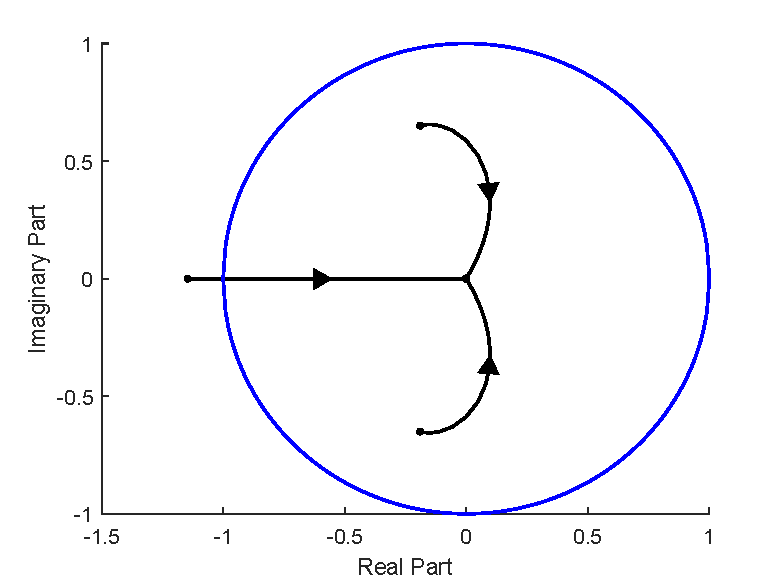
\includegraphics[width = 0.7\textwidth]{Chapter10_NMPC/LinearEigenvalueLocus.pdf}
\caption{Locus of closed loop eigenvalues (black) in the proposed MPC algorithm for a linear FIR example as $\Gamma_u$ varies from $0 \rightarrow \infty$. The closed loop system is unstable to begin with, but becomes stable once $\Gamma_u$ is large enough to bring all eigenvalues inside the unit circle (blue).}
\label{fig:LinearEigenvalueLocus}
\end{figure}

%\subsection{Second order case}
%
%In the case of a second order Volterra-Laguerre model, stability can again be guaranteed for large enough $\Gamma_u$, however the method of proof no longer allows direct computation of the threshold for a given model. The theorem and proof are as follows.
%
%\begin{thm}
%The statement in Theorem \ref{thm:LinearFIR_MPCStability} is still true if the system is instead described by a second order Volterra-Laguerre model, i.e. using (\ref{eqn:SS_dynamic_VL}) and (\ref{eqn:SS_output_VL}) with $M=2$.
%\label{thm:SecondOrder_MPCStability}
%\end{thm}
%
%\begin{proof*}
%From (\ref{eqn:MPC_finalminimizer}), we have that the applied input, $u^*(t)$, will be a \emph{real} root of the cubic polynomial,
%\begin{equation}
%\beta_3 [u(t)]^3 + \beta_2 [u(t)]^2 + (\beta_1 + \Gamma_u) [u(t)] + (\beta_0 - \Gamma_u u(t-1)) = 0,
%\end{equation}
%where $\beta_i = \sum_{j=1}^{p} \beta_{i,j}$ for $i = 0,1,2,3$.
%
%The cubic discriminant reveals that there will be only one real root if the following statement is true:
%\begin{equation}
%\Delta = ... <0
%\end{equation}
%In the discriminant, the highest power of $\Gamma_u$ appears with negative sign, thus we know $\exists \Upsilon \in \mathbb{R}^+$ such that $\Delta<0 \; \; \forall \Gamma_u > \Upsilon$. 
%
%Looking only at the $\Delta<0$ case now, the input $u^*(t)$ is found via
%
%\end{proof*}

\subsection{General case}

The analysis of stability for arbitrary order Volterra-Laguerre models is far more complex than in the linear case. The first issue is that it is not always possible to obtain an explicit control law from (\ref{eqn:MPC_finalminimizer}), since no analytic expressions exist for the roots of polynomials of order 5 and higher. Furthermore, even in cases where an analytic expression can be obtained there may be multiple real roots, and the resulting control laws will not be linear functions of the state vector in general.

However, we can still look at the limiting behaviour, where $\Gamma_u \rightarrow \infty$. In this case, (\ref{eqn:MPC_finalminimizer}) reduces to
\begin{align}
&u^*(t) \in   \Bigg\{ u(t): \Gamma_u u(t)  - \Gamma_u u(t-1) = 0 \Bigg\} \\
\implies & u^*(t) = u(t-1),
\end{align}
which is trivially stable, since the input is clearly bounded and the system model is stable by definition. This provides a level of confidence that the MPC algorithm will be stable for sufficiently large $\Gamma_u$.

\section{Conclusion}

A computationally efficient model predictive control algorithm was proposed in this chapter for systems modeled using the Laguerre-expanded Volterra series. A flexible state space modeling framework was developed to represent Volterra-Laguerre systems of any nonlinear order, then a typical quadratic objective function was employed, with arbitrary prediction horizon and a move horizon of 1. The move horizon was restricted in order to reduce the MPC optimization problem to a polynomial root-finding problem, the solution of which can be computed efficiently online. Suggested modifications to the algorithm were also provided in order to handle input constraints and enable offset-free reference tracking in steady-state. Finally, the stability of the proposed algorithm was investigated, where the linear case in particular highlights the importance of an appropriately scaled input penalty in the MPC objective function.